\documentclass[english]{upeeei}
\usepackage[latin9]{inputenc}
\setcounter{secnumdepth}{3}
\setcounter{tocdepth}{3}
\usepackage[active]{srcltx}
\usepackage{float}
\usepackage{units}
\usepackage{graphicx}

\makeatletter

\providecommand{\LyX}{L\kern-.1667em\lower.25em\hbox{Y}\kern-.125emX\@}
\providecommand{\tabularnewline}{\\}

\@ifundefined{showcaptionsetup}{}{%
 \PassOptionsToPackage{caption=false}{subfig}}
\usepackage{subfig}
\makeatother

\usepackage{babel}
\begin{document}

\title{Development of a 3D-Printed Quadrupedal Robot with Distributed Joint Control} 

\author{
Jiego Benjamin Osea Guanzon\\ 2015-07906\\ \emph{B.S. Electronics and Communications Engineering}
\and
}

%%
%% Month and year of submission/graduation
\degreeyear{2019} 
\degreesemester{December} 

% Put your advisers here:
\chair{Nicollete Arriola} 
\othermembers{Manuel Ramos}
\numberofmembers{2} 

\field{Electrical/Computer/Electronics and Communications Engineering} 
\campus{Diliman} 

\maketitle 
% \approvalpage 
% \copyrightpage 
\begin{abstract} 

In a \emph{single} well-written paragraph, this is what we'd like to do.  Try to cover Need, Solution, Differentiation, Benefit (NSDB).  Use the content of this template as an example for formatting your proposal document, \textbf{NOT} as a strict guide for the flow of your discussion and what your proposal must contain.

\abstractsignature\end{abstract}

\begin{frontmatter} 

\setlength{\parskip}{0pt}

\tableofcontents{}

\listoffigures

\listoftables

\end{frontmatter} 

\def\MASTERDOC{true}

\cleardoublepage{}

\chapter{Introduction\label{cha:Introduction}}

\section{Background of the Project}

Legged robots have several advantages over other types of mobile robots. While wheeled robots can move at high speeds, their operation is limited to relatively flat environments. Legged robots, on the other hand, have higher degrees of freedom (DOF) allowing them to operate in uneven and unpredictable terrain. Discrete motion trajectories and multiple limbs translate to higher maneuverability and flexibility coupled with stability and fault tolerance \cite{quadrobotlegs}.

However, bipedal (two-legged) robots have periods of instability during locomotion where only one leg is in contact with the ground. Other configurations with three or more legs have the characteristic of being stable as long as their center of mass is within the support polygon defined by the position of their legs. While having more legs usually means higher stability, it has the drawback of requiring more actuators and having more complex gaits. Quadrupedal robots, or four-legged robots, offer a robust middle-ground platform that has better load capacity and higher stability than bipedal robots while using fewer actuators compared to higher leg-count robots \cite{quadrobotlegs}.

Quadrupedal robots, such as Boston Dynamic's Bigdog \cite{bigdog} and MIT's Cheetah 3 \cite{cheetah3}, are generally inaccessible to most researchers due to their high cost and large size. MIT's state-of-the-art Mini Cheetah \cite{minicheetah} is a low-cost version of its predecesor, the Cheetah 3 robot. It has a small form-factor, approximately 60\% of the Cheetah 3 robot, and costs approximately \$3600. While the cost is significantly smaller than its predecessor, it is still too expensive for most experimental and research purposes.

\section{Project Objectives}

The project aims to develop a prototype of a cost-efficient 12-DOF quadrupedal robot. Proprioceptive actuators, with off-the-shelf brushless DC (BLDC) motors, are used to drive the joints to allow locomotion in uneven terrain. Custom joint controllers are to be used with the proprioceptive actuators while a custom main controller is to be used to handle the entire robot.

The project also aims to create a robust platform that is to be used with gait experimentation and other quadrupedal robot research.

\section{Project Overview}

The project can be divided into two major parts: design and control. The block diagram of the project is shown in Figure X below.

\subsection{Design}

The design part of the project can be further divided into two parts: mechanical and electronics design. 

Mechanical design of the quadrupedal robot involves the modelling and construction of the actuator, joints, legs, and body of the robot. Modelling is done and simulated using Fusion360. Fused Deposition Modelling (FDM) 3D-printing is used to fabricate each part with polylactic acid (PLA). The actuator is comprised of a BLDC motor coupled to a 6.125 reduction ratio 3D-printed planetary gearbox. The joints are driven either directly by the actuator or by a timing belt.

Electronics design of the quadrupedal robot involves the design and fabrication of custom main and joint controllers (WHAT TOPOlOGY?). Both controllers utilize a dsPIC33 microcontroller while the joint controller has a smart gate driver integrated circuit (IC) which drives a three-phase power inverter. The method of power delivery to each actuator is also considered in this design phase.

\subsection{Control}

The control part of the project can be further divided into three parts: joint, stability, and gait control.

Joint control, which is local to each motor controller, is responsible for the low level control of output torque and speed of each actuator. Stability control is responsible for the overall balance of the robot. Gait control is responsible for generating the trajectories of each leg and sending positional and velocity data setpoints to each actuator. Both stability and gait control are processed by the main microcontroller of the quadruped.

\section{Documentation Flow and Organization}

Chapter 2 discusses different types of commonly used mechanical legs for quadrupeds along with the different types of actuators that drive them. Materials, along with their advantages and disadvantages, are also discussed in the chapter. Finally, a few control algorithms and structures are discussed.

Chapter 3 states the project's main objectives and discusses the problems it aims to solve.

\cleardoublepage{}

\chapter{Related Work\label{cha:RRW}}

\section{Actuators}

\section{Mechanical Legs}

The most essential part of a quadrupedal robot are its mechanical legs. Their design and topology determines the overall performance and behavior of the robot since it defines its effective maneuverability, walking speed, and load capacity \cite{designprinciples}. There are three types of mechanical legs that are commonly used by quadrupeds: prismatic, articulated, and redundant articulated legs. 

Prismatic legs are the simplest type of mechanical legs since they only have a single rotating joint and a prismatic joint as shown in Figure \ref{fig:prismatic-leg} \cite{quadrobotlegs}. 

\begin{figure}[H]
\begin{centering}
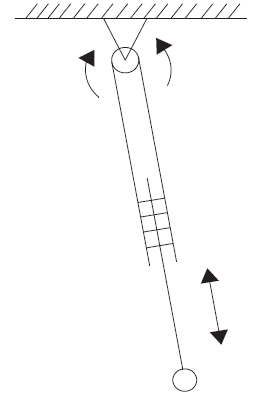
\includegraphics[width=0.3\columnwidth]{images/prismatic_leg}
\par\end{centering}
\caption{Prismatic Leg Topology\label{fig:prismatic-leg}}
\end{figure}

This type of leg typically mimics the bounce and compliance of an animal's leg with its prismatic joint using different kinds of springs. The work of Raibert et al. used a hydraulic actuator that is in series with an air spring, shown in Figure \ref{fig:quad-running-robot}, to control the leg length while still having compliance from the spring \cite{quadrunningrobot}. The Scout II quadrupedal robot, made by Poulakakis et al., uses only passive springs in its design for its prismatic legs which is shown in Figure \ref{fig:scout-ii} \cite{quadrobotlegs, scoutii}.

\begin{figure}[H]
\begin{centering}
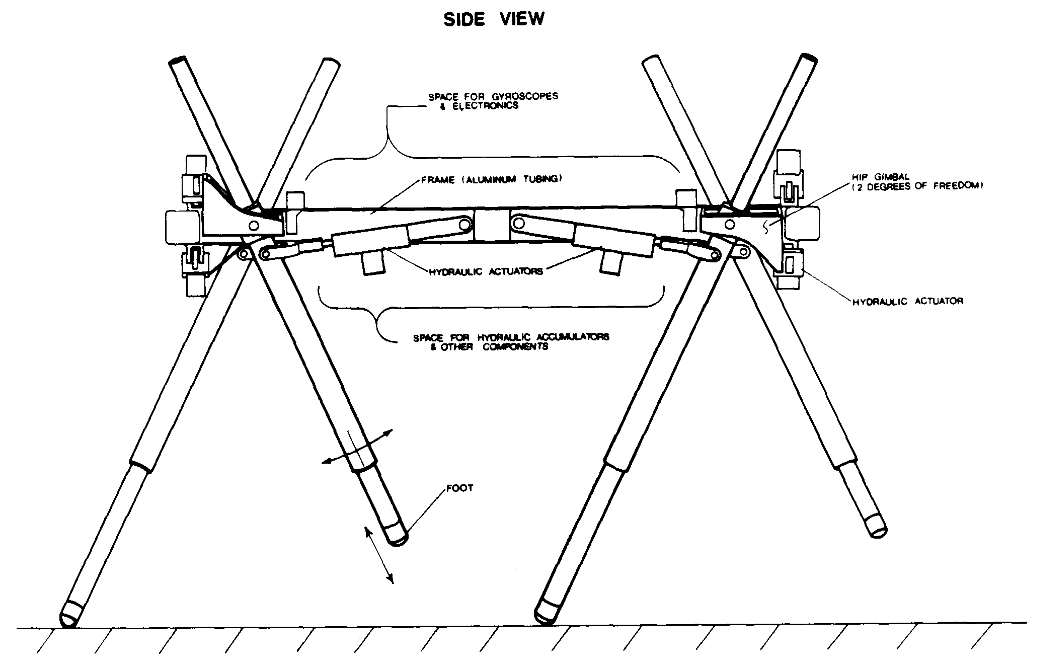
\includegraphics[width=0.75\columnwidth]{images/quad_running_robot}
\par\end{centering}
\caption{Four-legged Running Machine\label{fig:quad-running-robot}}
\end{figure}

\begin{figure}[H]
\begin{centering}
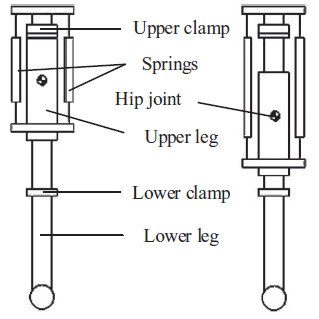
\includegraphics[width=0.3\columnwidth]{images/scout_ii}
\par\end{centering}
\caption{Scout II Robot\label{fig:scout-ii}}
\end{figure}

Prismatic legs are lightweight and have low inertia which is ideal for high-speed locomotion. Due to some designs using passive spring systems, less energy has to be expended to actuate the legs therefore high-efficiency movement can be achieved. They are also innately impact-resistant and provide fixed compliance to outside forces acting on it.

The second type of mechanical legs is the articulated leg. This leg topology replaces the prismatic joint of the prismatic leg with a rotational joint, similar to a knee or elbow joint, giving it a total of two rotational joints. This topology is a better representation, compared to the prismatic leg, of a typical leg structure of a natural four-legged animal. Control of the leg length is done by actuation of each rotational joint in conjunction with each other. The topology of the leg joints is shown in Figure \ref{fig:articulated-leg} \cite{quadrobotlegs}. 

\begin{figure}[H]
\begin{centering}
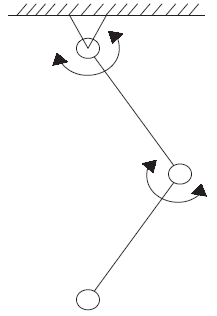
\includegraphics[width=0.3\columnwidth]{images/articulated_leg}
\par\end{centering}
\caption{Articulated Leg Topology\label{fig:articulated-leg}}
\end{figure}

There are two types of configuration of articulated legs on a quadruped: mammal and sprawling configuration. Mammal configurations have their legs positioned vertically with respect to the robot while sprawling configuration have the first segment of the leg (thigh) positioned horizontal with respect to the robot and the second leg segment (shank) being vertical. The topologies of both configurations are shown in Figure \ref{fig:articulated-configurations} \cite{titanxiii}.

\begin{figure}[H]
\begin{centering}
\subfloat[Mammal Configuration]{\begin{centering}
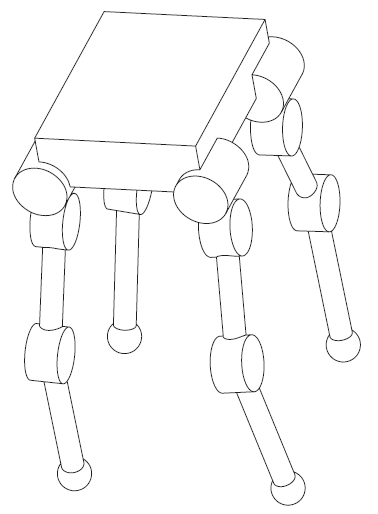
\includegraphics[width=0.25\columnwidth]{images/mammal_articulated}
\par\end{centering}
}
\par\end{centering}
\begin{centering}
\subfloat[Sprawling Configuration]{\begin{centering}
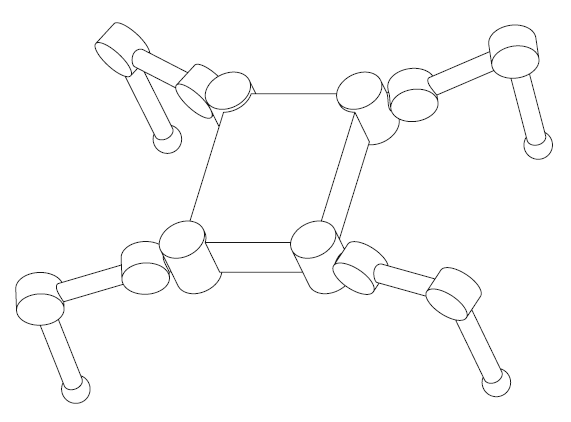
\includegraphics[width=0.4\columnwidth]{images/sprawling_articulated}
\par\end{centering}
}
\par\end{centering}
\caption{Articulated Leg Configurations\label{fig:articulated-configurations}}
\end{figure}

Mammal configurations are often more compact and have a smaller footprint, with the added benefit of requiring low joint torques with the legs bent. On the other hand, sprawling configurations are typically more stable due to its large stability polygon and the ability to lower its center of gravity without affecting its locomotion. This configuration, however, has several disadvantages compared to the mammal configuration. Sprawling configurations require the pitch axis to continuously generate torque to support its own weight, therefore reducing its efficiency. They also move significantly slower than mammal configurations.

Semini et al. have developed three quadrupedal robots with articulated legs, namely: HyQ, HyQ2Max, and MiniHyQ. The HyQ quadrupedal robot uses electro-hydraulic actuated legs. This system combines the high torque output of hydraulic actuators with the space-efficiency and high-speed of electric actuators to provide high power-to-weight ratio, high actuation speed, and torque robustness. The thigh of the robot is composed of parallel ribs that are linked together keeping it lightweight and low inertia. The shank is a cylindrical structure that houses an additional passive prismatic ankle joint. The topology of the HyQ robot leg is shown in Figure \ref{fig:hyq-leg} \cite{quadrobotlegs, hyq}.

\begin{figure}[H]
\begin{centering}
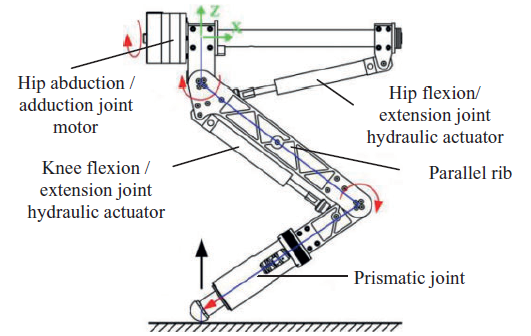
\includegraphics[width=0.7\columnwidth]{images/hyq}
\par\end{centering}
\caption{HyQ Leg Topology\label{fig:hyq-leg}}
\end{figure}

The HyQ2Max quadrupedal robot builds upon the HyQ with higher joint torques and payload, faster movement, and wider range of motion while maintaining the use of hydraulic actuators \cite{hyq2max}. The MiniHyQ quadrupedal robot builds upon the previous two models. Despite the name, it has the same leg length as the HyQ but with less weight and higher range of motion. The leg topology of the MiniHyQ is shown in Figure \ref{fig:mini-hyq-leg} \cite{minihyq}.

\begin{figure}[H]
\begin{centering}
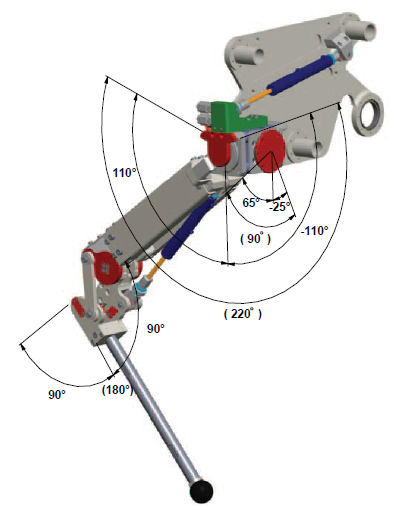
\includegraphics[width=0.3\columnwidth]{images/minihyq}
\par\end{centering}
\caption{MiniHyQ Leg Topology\label{fig:mini-hyq-leg}}
\end{figure}

\begin{figure}[H]
\begin{centering}
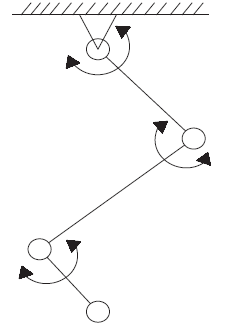
\includegraphics[width=0.3\columnwidth]{images/redundant_articulated_leg}
\par\end{centering}
\caption{Redundant Articulated Leg Topology\label{fig:redundant-articulated-leg}}
\end{figure}

\section{Materials}
\section{Control}

\cleardoublepage{}

\chapter{Problem Statement and Objectives \label{cha:ProbStatement}}

The problem statement and objectives are placed on a separated chapter
for project proposals after the review of related work. The previous
chapter builds up the foundation of the project by highlighting the
advantages and disadvantages of the relevant related work. The main
problem that the project intends to solve is then presented in this
chapter. The project objectives should also be discussed here.

\cleardoublepage{}

\chapter{Methodology\label{cha:Methodology}}

\section{Design and Implementation}
\subsection{Mechanical}

The quadrupedal robot implements three Degrees of Freedom (DOF) per leg. Two DOF joints are used for the hips which control the abduction/adduction and flexion/extension motion. One DOF joints are used for the knee to control its flexion/extension motion. No joints are designed into the quadruped's ankles since the actuators are backdrivable and force-compliant.  Fusion360 is used to design and simulate the quadruped. The 3D model of the robot is shown in Figure X below.

Each joint will be driven by an actuator that consists of a BLDC motor coupled to a single state planetary gearbox. The planetary gearbox has a reduction ratio of 6.125 which makes the actuator quasi-direct drive. Each actuator including the planetary gearbox will be 3D printed using readily available polylactic acid (PLA). Bearings are added to provide smoother rotation rotation of gears and more even distribution of loads, while threaded inserts are used to have stronger points to screw on. The actuator has an overall diameter of 110 mm and length of 75 mm and weighs 700 grams in total. An exploded view of the joint actuator is shown in Figure X below.

The three joint actuators for each leg are designed to be mounted at the top of the legs and as close to the body as possible. This makes sure that the actual legs would be as light as possible to minimize the leg's inertia. The two hip joints are directly coupled to the actuator using a 3D printed joint connector. The knee joint, on the other hand, uses a timing belt coupled to the output of the knee actuator to control the knee, providing an additional 1.25 gear reduction ratio. This configuration allows the robot's hips to have 180 degrees of rotation about its own roll axis and 360 degrees about its pitch axis. The robot's knees have 270 degrees of rotation. 

The quadruped's legs consists of two links: upper and lower link. The upper link consists of two halves, connected to each other using screws, to enable access to the timing belt during assembly and maintenance. The lower link is one solid part that has a gear at one of its end and revolves around the lower part of the upper link. Lastly, the foot is a round object made out of rubber to absorb small amount of forces and provide some compliance.

The hip abduction/adduction actuators are mounted onto the 3D printed body. The body houses the main controller of the robot and the battery to power the robot. The overall size of the quadrupedal robot is UxV mm.

\subsection{Electronics}

The quadrupedal robot uses a custom designed joint controller and main controller board. The joint controller is responsible with controlling the brushless DC (BLDC) motor in the actuator while the main controller is responsible with trajectory generation and propagation of positional data for the joints. Both controller boards are designed around Microchip's dsPIC33CK family of digital signal controllers (DSCs). The specific model and features of the DSCs used are shown in Table X below.

The joint controller is made up of four main compontents: microcontroller, gate driver, output stage, and encoder. The microcontroller used is the dsPIC33CK128MP505. The gate driver used is Texas Instruments' DR8323 Three-Phase Smart Gate Driver. This gate driver is responsible for driving an external three-phase inverter stage that generates the sinusoidal voltages used to drive the motor. The three-phase inverter stage uses the N-channel NTMFS4935NT1G MOSFETs which are rated for 30V and 13A. Lastly, the controller uses an AS5047P magnetic rotary position sensor, that is mounted at the back of the printed circuit board (PCB), to sense the rotation of the BLDC rotor and track its position and speed with 14 bits of resolution. Shunt resistors are  added onto the board in order to measure the current in each phase of the motor. Other needed components such as resistors, capacitors, inductors, diodes, and terminals are also designed into the controller upon recommendation of each main components' datasheets. Schematic capture and PCB layout design for both the joint and main controller was done on KiCad. Top and bottom layers of the 2-layer joint controller PCB are shown in Figures X and Y respectively.

The main controller is mainly composed of the dsPIC33CK128MP508 microcontroller. This microcontroller comes in the 80 TQFP package. The board also features 12 terminals for the CAN bus connections of each actuator. UART breakout pins are also added for communication to a PC. Top and bottom layers of the 2-layer main controller PCB are shown in Figures X and Y respectively.

\subsection{Control}

Control in the quadrupedal robot can be divided into three parts: joint, stability, and gait control. Each part is independent but functions in conjuction with the others.

Joint control of the quadruped is distributed across the joint controllers of each actuator. It is responsible for controlling the torque and commutation of the BLDC motor in the actuator. It accepts positional data from the main controller and uses the Field Oriented Control (FOC) algorithm to generate three-phase sinusoidal voltages that maximize the torque output of the BLDC motor. The block diagram for the FOC algorithm is shown in Figure X below.

The first step in FOC is measuring the current of two phases of the motor and computing for the third using Equation X. 

Clarke Transform is applied to the three-phase currents that is referenced to the stator and moves them onto a 2D orthogonal system, still referenced to the stator, called alpha-beta.

Park Transform is applied to the two-phase, stator-referenced currents and rotates them onto the d-q coordinate system that is referenced to the rotor. The two-phase currents are now treated as DC signals and can be controlled using conventional Proportional-Integral (PI) controllers. 

Error signals are generated for the position, speed, Iq, and Id currents and are fed through individual cascaded PI controllers. The rotor angle and rotor speed are computed using an observer shown in Figure X below. 

The Vq and Vd outputs from the respective Iq and Id PI controllers are then referenced back onto the stator using the Inverse Park Transform. 

The final step in FOC is to generate pulse-width modulation signals, with frequency of 20 kHz, for the three-phase inverter using Space Vector Modulation (SVM). SVM represent the six possible states of the three-phase inverter as space vectors which are 60 degrees apart. It calculates which sector the resultant voltage vector is in and achieves this voltage by varying, thus averaging, the time spent on the two adjacent space vector states. The duty cycles are calculated and updated. The algorithm is done every Analog-to-Digital Converter (ADC) interrupt which is triggered by the PWM module.

\section{Testing}

SPECIFY TARGET RESULTS

The actuator's torque output with varying current is to be tested by attaching a link with a length of 200 mm directly to its output carrier and measuring the maximum weight it can support without failure. The torque vs current is to be graphed alongside with the calculated torque constant. The actuator's thermal performance is to be tested by running the BLDC motor at its maximum rated speed for a set amount of time and measuring the temperature of the actuator using a thermal imaging camera or a thermocouple.

Tuning of the PI controllers is to be done empirically. For the FOC, the inner PI controllers are to be tuned first before the outer controllers. Step response of the joint actuators to torque, current, speed, and position set points are to be tested and verified. Testing of each leg is to be done before assembly of the quadruped. Static gaits is to be fed to the quadruped robot to test its initial stability.

\cleardoublepage{}

\chapter{Preliminary Findings\label{cha:Prelims}}

This is an optional chapter where you present all of your preliminary
work, results, and analysis. For final project documentations, this
chapter becomes the Results and Analysis chapter.

\cleardoublepage{}

\chapter{Project Schedule and Deliverables\label{cha:Project-Sked}}

For final project documentations, this chapter becomes the Conclusions
and Recommendations chapter.

For project proposals, end the documentation by presenting the project
schedule and expected deliverables. This section should clearly describe
the activities that will be done. Important milestones should be indicated
in the schedule of activities. It should be as specific as possible. 

\section{Gantt Chart }

This is a time table that clearly indicates the important milestones
of the project. The schedule should be divided into weekly segments.
The authors should make sure that the schedules are realistic. It
is advised that the weekly tasks are as detailed as possible. 

\section{Halfway-point Deliverables}

This section should clearly point out and describe the expected outputs
at halfway-point. If the project will be done by a group, the deliverables
of each group member shall be clearly and specifically stated. 

\section{Final Deliverables}

This section should clearly point out the final deliverables. If the
project will be done by a group, the deliverables of each group member
shall be clearly and specifically stated.

\cleardoublepage{}

\bibliographystyle{unsrt}
\nocite{*}
\bibliography{bibliography}

\cleardoublepage{}

\appendix

\chapter{Appendices}

If there is only one appendix, it shall be labeled \textquotedblleft Appendix:\textquotedblright{}
and the appendix title. If there are more than one appendices, they
shall be labeled \textquotedblleft Appendix A: {[}title{]}\textquotedblright ,
\textquotedblleft Appendix B: {[}title{]}\textquotedblright , etc.
For software projects, appendices may include program listings, screen
shots, and sample input and output files. For hardware projects, appendices
may include printed circuit board layouts and geometric design layouts.
Other possible appendices include user manuals (created by the author
for the project), long mathematical proofs, and reviews of basic concepts.

You can insert appendices through the \textbf{Document \textgreater{}
Start Appendix Here} option. The appendix should start after the bibiliography
section of the main document. Appendices can also have chapters and
sections. \LyX{} automatically lists the appendices alphabetically.

\cleardoublepage{}

\chapter{Formatting Tips}

\section{Inserting Chapters}

On the upper left dropdown menu of the \LyX{} window, select \textit{Chapter}.
You can then type the chapter title that you want. Pressing Enter
will revert the format to \textit{Standard}, where the content can
now be placed. Chapters are numbered and placed on the \textit{Table
of Contents} automatically.

\section{Inserting Sections}

On the same dropdown menu where you insert a chapter, select \textit{Sections}.
The sections under the chapter are automatically numbered accordingly.
These also appear in the generated \textit{Table of Contents}.

\subsection{Subsections}

You can also add subsections and subsubsections. However, use them
sparingly, especially the latter.

\section{Inserting Labels}

On the chapter/section/image/table that you want to reference, click
\textbf{Insert \textgreater{} Label}. You can use the default label
that \LyX{} generates for you. To 'call' it anywhere in your document,
click the \textbf{Insert \textgreater{} Cross-reference}. This provides
an efficient way of pointing out figure/table and chapter/section
numbers, without the need to type out explicitly what the numbers
are in the document.

\section{Inserting Floats}

Figures and tables shall be included in the body of the documentation
to illustrate or clarify the accompanying text. Thus, figures and
tables must be referenced in the text in order for them to be meaningful.
By convention, figure names should be placed below the image, while
table names should be placed on top of the table. 

Moreover, figures or tables should not appear in the document before
they are mentioned in the text. By default, \LyX{} does not follow
this rule and places images or tables near, but not exactly after,
the text referencing it. You can force the rule by right-clicking
on the \textit{float:Figure} label in the \LyX{} editor and going to
\textit{Settings}. In the window that appears, shown in Figure \ref{fig:Forcing-float-placement},
uncheck \textit{Use default placement} and check \textit{Here definitely}
instead.

\begin{figure}[H]
\begin{centering}
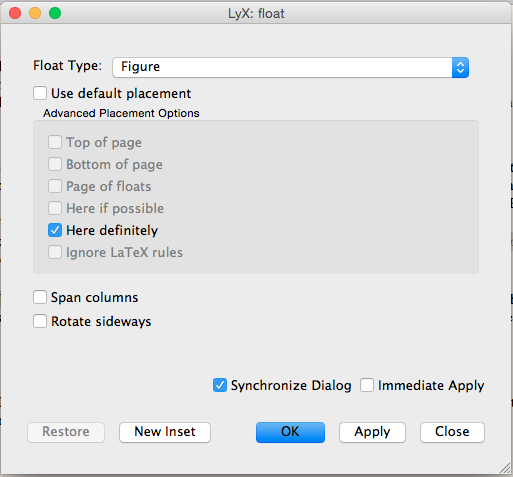
\includegraphics[width=0.5\columnwidth]{images/placement}
\par\end{centering}
\caption{Forcing float placement\label{fig:Forcing-float-placement}}

\end{figure}


\subsection{Inserting Images}

Place your cursor on the area where you want to insert the image.
Select \textbf{Insert \textgreater{} Float \textgreater{} Figure}.
Insert the actual image by selecting \textbf{Insert \textgreater{}
Graphics}. It is a recommended practice that all images should be
placed on a single folder on the same directory of this \LyX{} document
template.

You can also center the image by putting first your cursor on the
side of the image that you want to center. Right click then select
\textit{Paragraph Settings}. Finally, select the \textit{Center} button. 

You can scale the images inside the document by clicking on the image.
As shown in Figure \ref{fig:LyX-Graphics-options}, images can be
scaled relative to the column width. For two column document formats,
scale the image relative to the text width.

\begin{figure}[H]
\begin{centering}
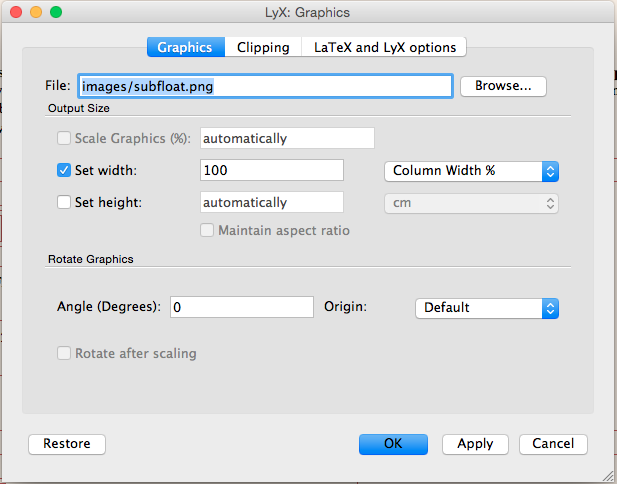
\includegraphics[width=0.6\columnwidth]{images/image_scale}
\par\end{centering}
\caption{\protect\LyX{} Graphics options\label{fig:LyX-Graphics-options}}

\end{figure}

As shown in Figure \ref{fig:Subfloat-Sample}, we can also insert
floats within the float. To put the subfloat to the document center,
click on the side of the \textit{subfloat: Figure} field, instead
of the image within the subfloat, and then access the \textit{Paragraph
Settings} as described in the previous steps. 

\begin{figure}[H]
\begin{centering}
\subfloat[Subfloat A]{\begin{centering}
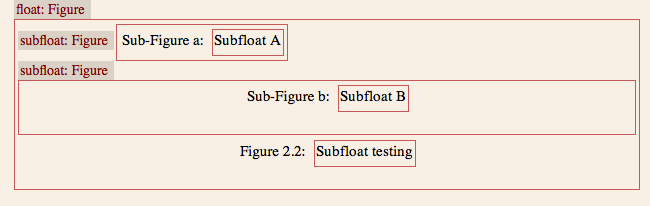
\includegraphics[width=0.8\columnwidth]{images/subfloat}
\par\end{centering}
}
\par\end{centering}
\begin{centering}
\subfloat[Subfloat B]{\begin{centering}
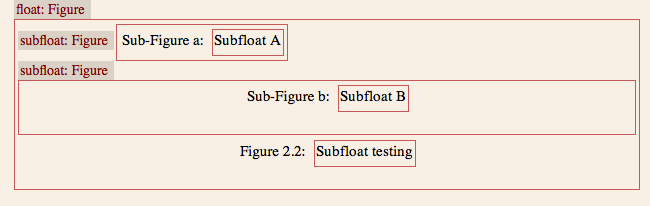
\includegraphics[width=0.8\columnwidth]{images/subfloat}
\par\end{centering}
}
\par\end{centering}
\caption{Subfloat Sample\label{fig:Subfloat-Sample}}
\end{figure}


\subsection{Inserting Tables}

Tables can be inserted just like Figure floats. Tables can also be
centered just like the images in the same way. Note that some tables
might be too long to fit the page. Again, by convention, table descriptions
are placed on top of tables as demonstrated in Table \ref{tab:Sample-Table}.
Make it fit by setting the column width (\textbf{Right click the whole
column -\textgreater{} More -\textgreater{} Settings}). 

\begin{table}[H]
\caption{Sample Table \label{tab:Sample-Table}}

\centering{}%
\begin{tabular}{|c|c|c|c|c|}
\hline 
Row 1, Column 1 & Row 1, Column 2 & Row 1, Column 3 & Row 1, Column 4 & Row 1, Column 5\tabularnewline
\hline 
\hline 
 &  &  &  & \tabularnewline
\hline 
 &  &  &  & \tabularnewline
\hline 
 &  &  &  & \tabularnewline
\hline 
 &  &  &  & \tabularnewline
\hline 
\end{tabular}
\end{table}


\section{Inserting Citations}

To download the Bib\TeX{} formatted citation from IEEEXplore, see Figure
\ref{fig:BibTeX-from-IEEEXplore}.

\begin{figure}[H]
\begin{centering}
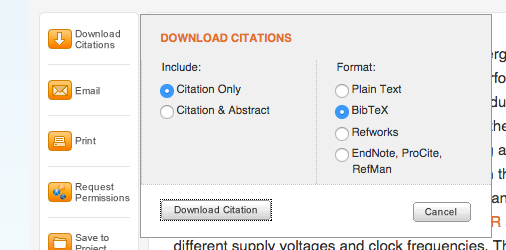
\includegraphics[width=0.55\columnwidth]{images/bibtex}
\par\end{centering}
\caption{Bib\protect\TeX{} from IEEEXplore\label{fig:BibTeX-from-IEEEXplore}}
\end{figure}

Put whatever text returned by IEEEXplore to your Bib\TeX{} file (.bib).
The references should follow the Bib\TeX{} format. To cite your paper
, click \textbf{Insert \textgreater{} Citation}, select
the desired paper, then click \textit{Add}, see Figure \ref{fig:Selecting-citations}. 

\begin{figure}[H]
\begin{centering}
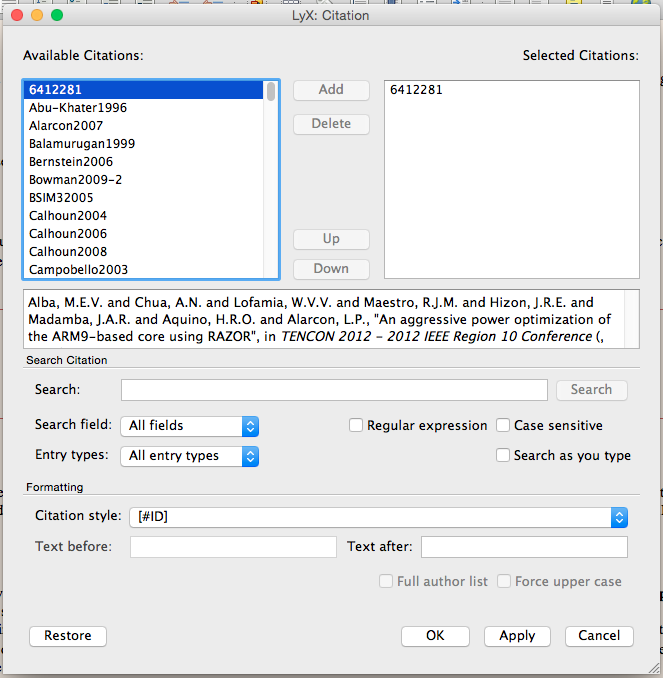
\includegraphics[width=0.7\columnwidth]{images/papers}
\par\end{centering}
\caption{Selecting citations \label{fig:Selecting-citations}}

\end{figure}

As shown in Figure \ref{fig:Bibliographies-with-no}, work titles
on bibliographies generated by Bib\TeX{} are not automatically capitalized.
Capitalization can be forced by editing the Bib\TeX{} file (.bib) and
then enclosing the capital letters of the titles with \{\}, such as
``\textbf{title=\{An \{A\}ggressive \{P\}ower \{O\}ptimization of
the \{ARM9\}-based core using \{RAZOR\}\},}''.

\begin{figure}[H]
\begin{centering}

\includegraphics[width=1\columnwidth]{images/bibliography}
\par\end{centering}
\caption{Bibliographies with no auto-capitalization \label{fig:Bibliographies-with-no}}

\end{figure}


\section{Inserting Equations}

You can insert inline equations like this: $V=IR$\textbf{ }by going
to \textbf{Insert -\textgreater{} Math -\textgreater{} Inline Equation}.
You can also insert numbered equations through \textbf{Insert \textgreater{}
Math \textgreater{} Numbered Formula}. 
\begin{equation}
\nicefrac{x}{y}=\frac{x}{y}
\end{equation}

\begin{equation}
P(Z>1)=P(Z<0)=\frac{1}{2}\left[1+erf\left(\frac{Z-0.5}{\sqrt{2(0.18)}}\right)\right]=0.1193\label{eq:1}
\end{equation}

\begin{equation}
T_{P}=\frac{\left[10\unitfrac{bits}{preamble}+(4\unitfrac{bytes}{packet})(8\unitfrac{bits}{byte})\right](16\unitfrac{symbols}{bit})}{450\unitfrac{ksymbols}{second}}=1.493ms\label{eq:4-1}
\end{equation}

A math toolbar, as shown in Figure \ref{fig:Math-toolbar-for}, will
appear whenever you try to edit an equation field. This greatly helps
in creating professional-looking equations. It is required that all
equations appearing in the document be written out using this option.

\begin{figure}[H]
\begin{centering}
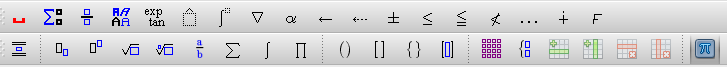
\includegraphics[width=0.9\columnwidth]{images/equations}
\par\end{centering}
\caption{Math toolbar for equation writing\label{fig:Math-toolbar-for}}

\end{figure}

\cleardoublepage
\end{document}
